\chapter{Circulator}

\section{Setup}

The DUT is a three-port circulator, a non-reciprocal RF device that routes signals directionally between its ports. Ideally, the circulator enforces a cyclic transmission of power:
\[
1 \rightarrow 2,\quad 2 \rightarrow 3,\quad 3 \rightarrow 1
\]

This means that a signal entering one port is transmitted only to the next port in the sequence, while the other port is ideally isolated.

Real circulators exhibit non-idealities such as insertion loss in the transmission path and finite isolation between non-connected ports.
\newpage
In order to characterize the device, two configurations were measured using a VNA:
\begin{itemize}
    \item \textbf{Configuration 1}: ports 1 and 2 connected to the VNA, with port 3 terminated by a matched $50\,\Omega$ load
    \item \textbf{Configuration 2}: ports 1 and 3 connected to the VNA, with port 2 terminated by a matched $50\,\Omega$ load
\end{itemize}

The matched termination is necessary to absorb the incoming power and avoid additional reflections from the unused port, which would otherwise modify the measured response.

\begin{figure}[H]
\centering
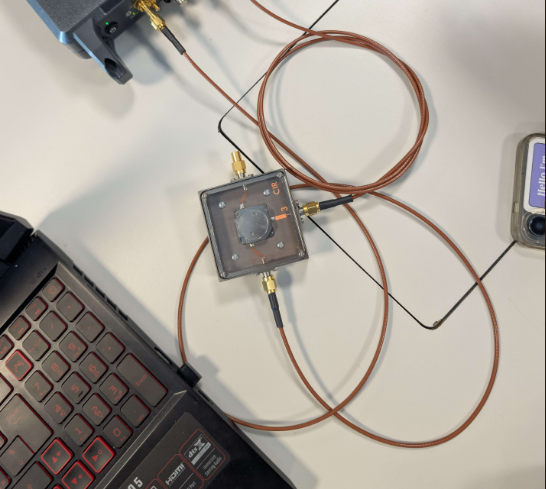
\includegraphics[height=0.5\textheight, width=0.45\textwidth, keepaspectratio]{Davides_Section/Circulator/plots/image.png}
\caption{Experimental setup used for the circulator characterization.}
\label{fig:circulator_setup}
\end{figure}

\section{Analysis of the Measurements}

\subsection{Configuration 1}

\begin{figure}[H]
\centering
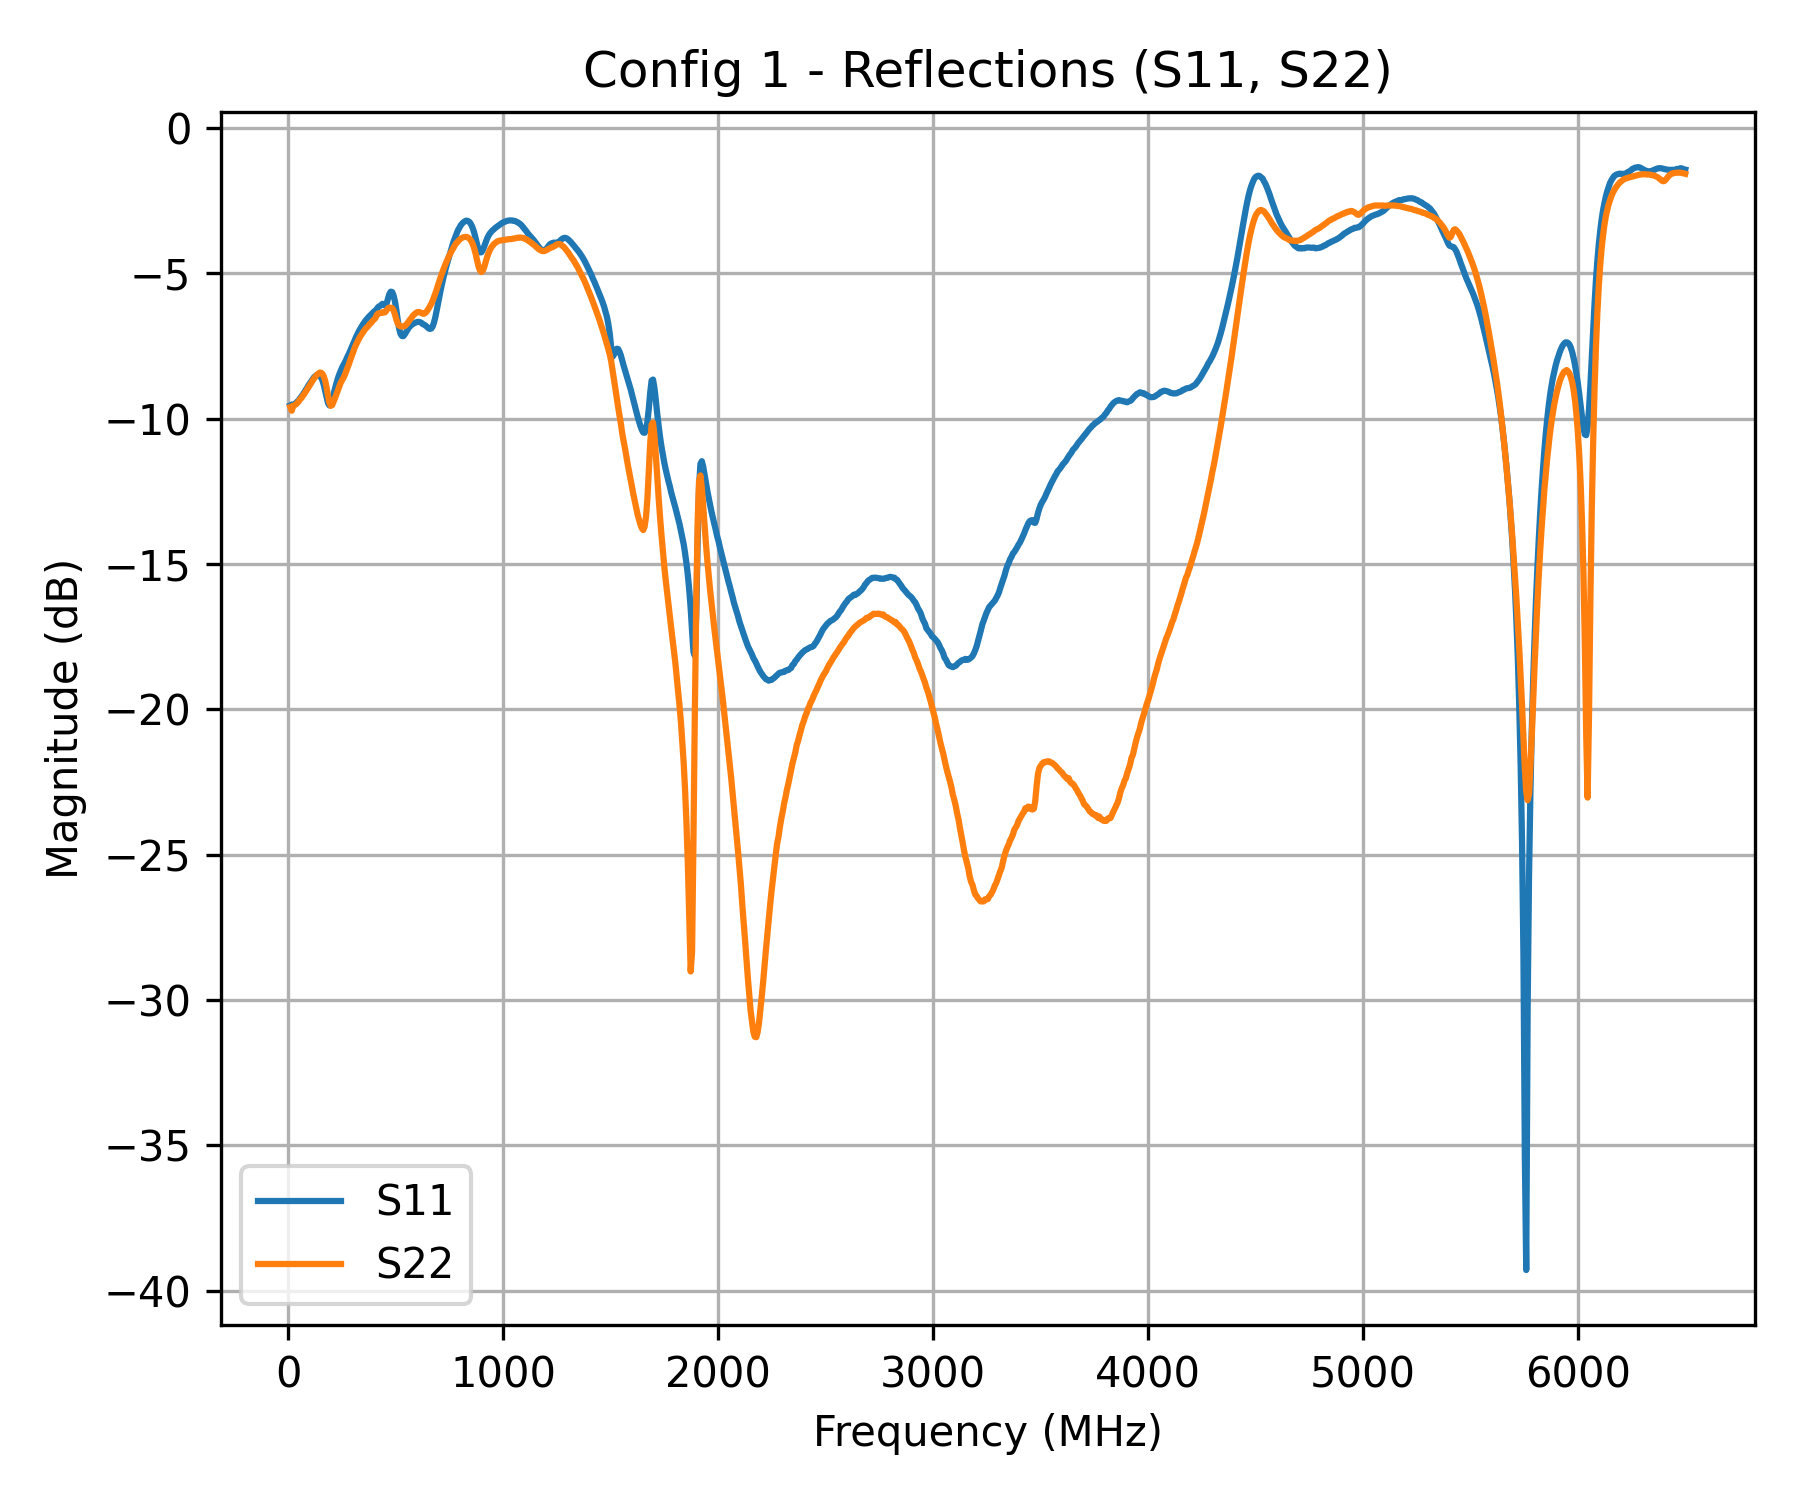
\includegraphics[width=0.6\linewidth]{Davides_Section/Circulator/plots/config1_reflection.png}
\caption{Reflection coefficients $S_{11}$ and $S_{22}$ for configuration 1.}
\label{fig:config1_reflection}
\end{figure}

The reflection coefficients $S_{11}$ and $S_{22}$ are generally below $-10\,\mathrm{dB}$ over a wide portion of the frequency range, indicating a reasonably good impedance matching at both measured ports. More pronounced minima are visible around the $2$--$3\,\mathrm{GHz}$ region, corresponding to frequencies where the device is better matched and therefore more efficient in transmitting power.

\begin{figure}[H]
\centering
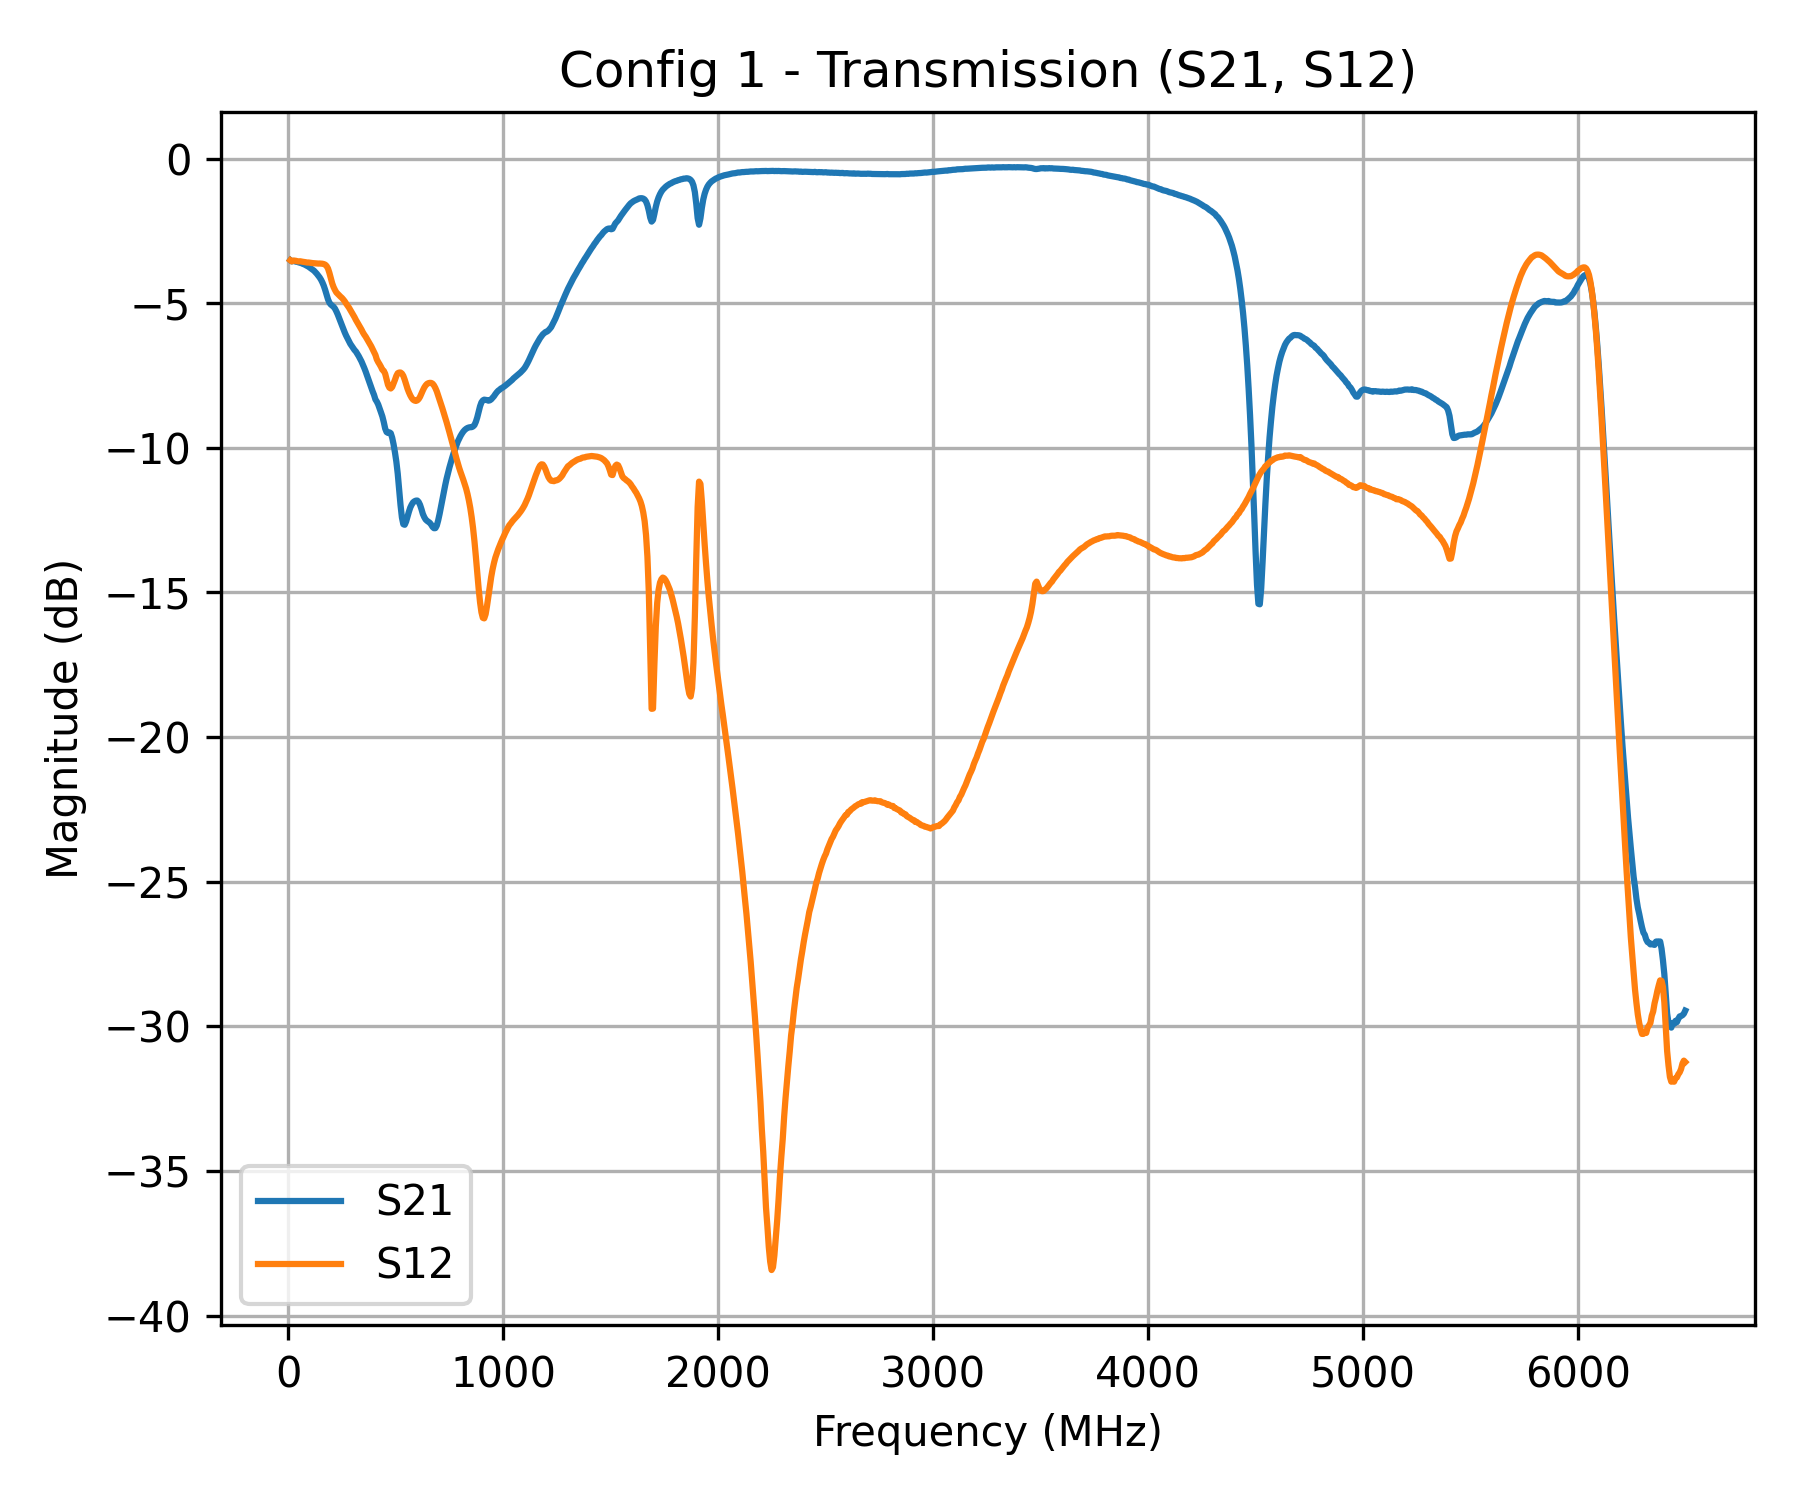
\includegraphics[width=0.6\linewidth]{Davides_Section/Circulator/plots/config1_transmission.png}
\caption{Transmission coefficients $S_{21}$ and $S_{12}$ for configuration 1.}
\label{fig:config1_transmission}
\end{figure}

The transmission response clearly shows the non-reciprocal behavior of the device. In this configuration, $S_{21}$ remains close to $0\,\mathrm{dB}$ over a broad frequency interval, meaning that power injected into port 1 is efficiently transferred to port 2. On the contrary, $S_{12}$ is much smaller and reaches strongly attenuated values, showing that the reverse propagation is suppressed. This is the expected behavior for the allowed transmission path $1 \rightarrow 2$.

\subsection{Configuration 2}

\begin{figure}[H]
\centering
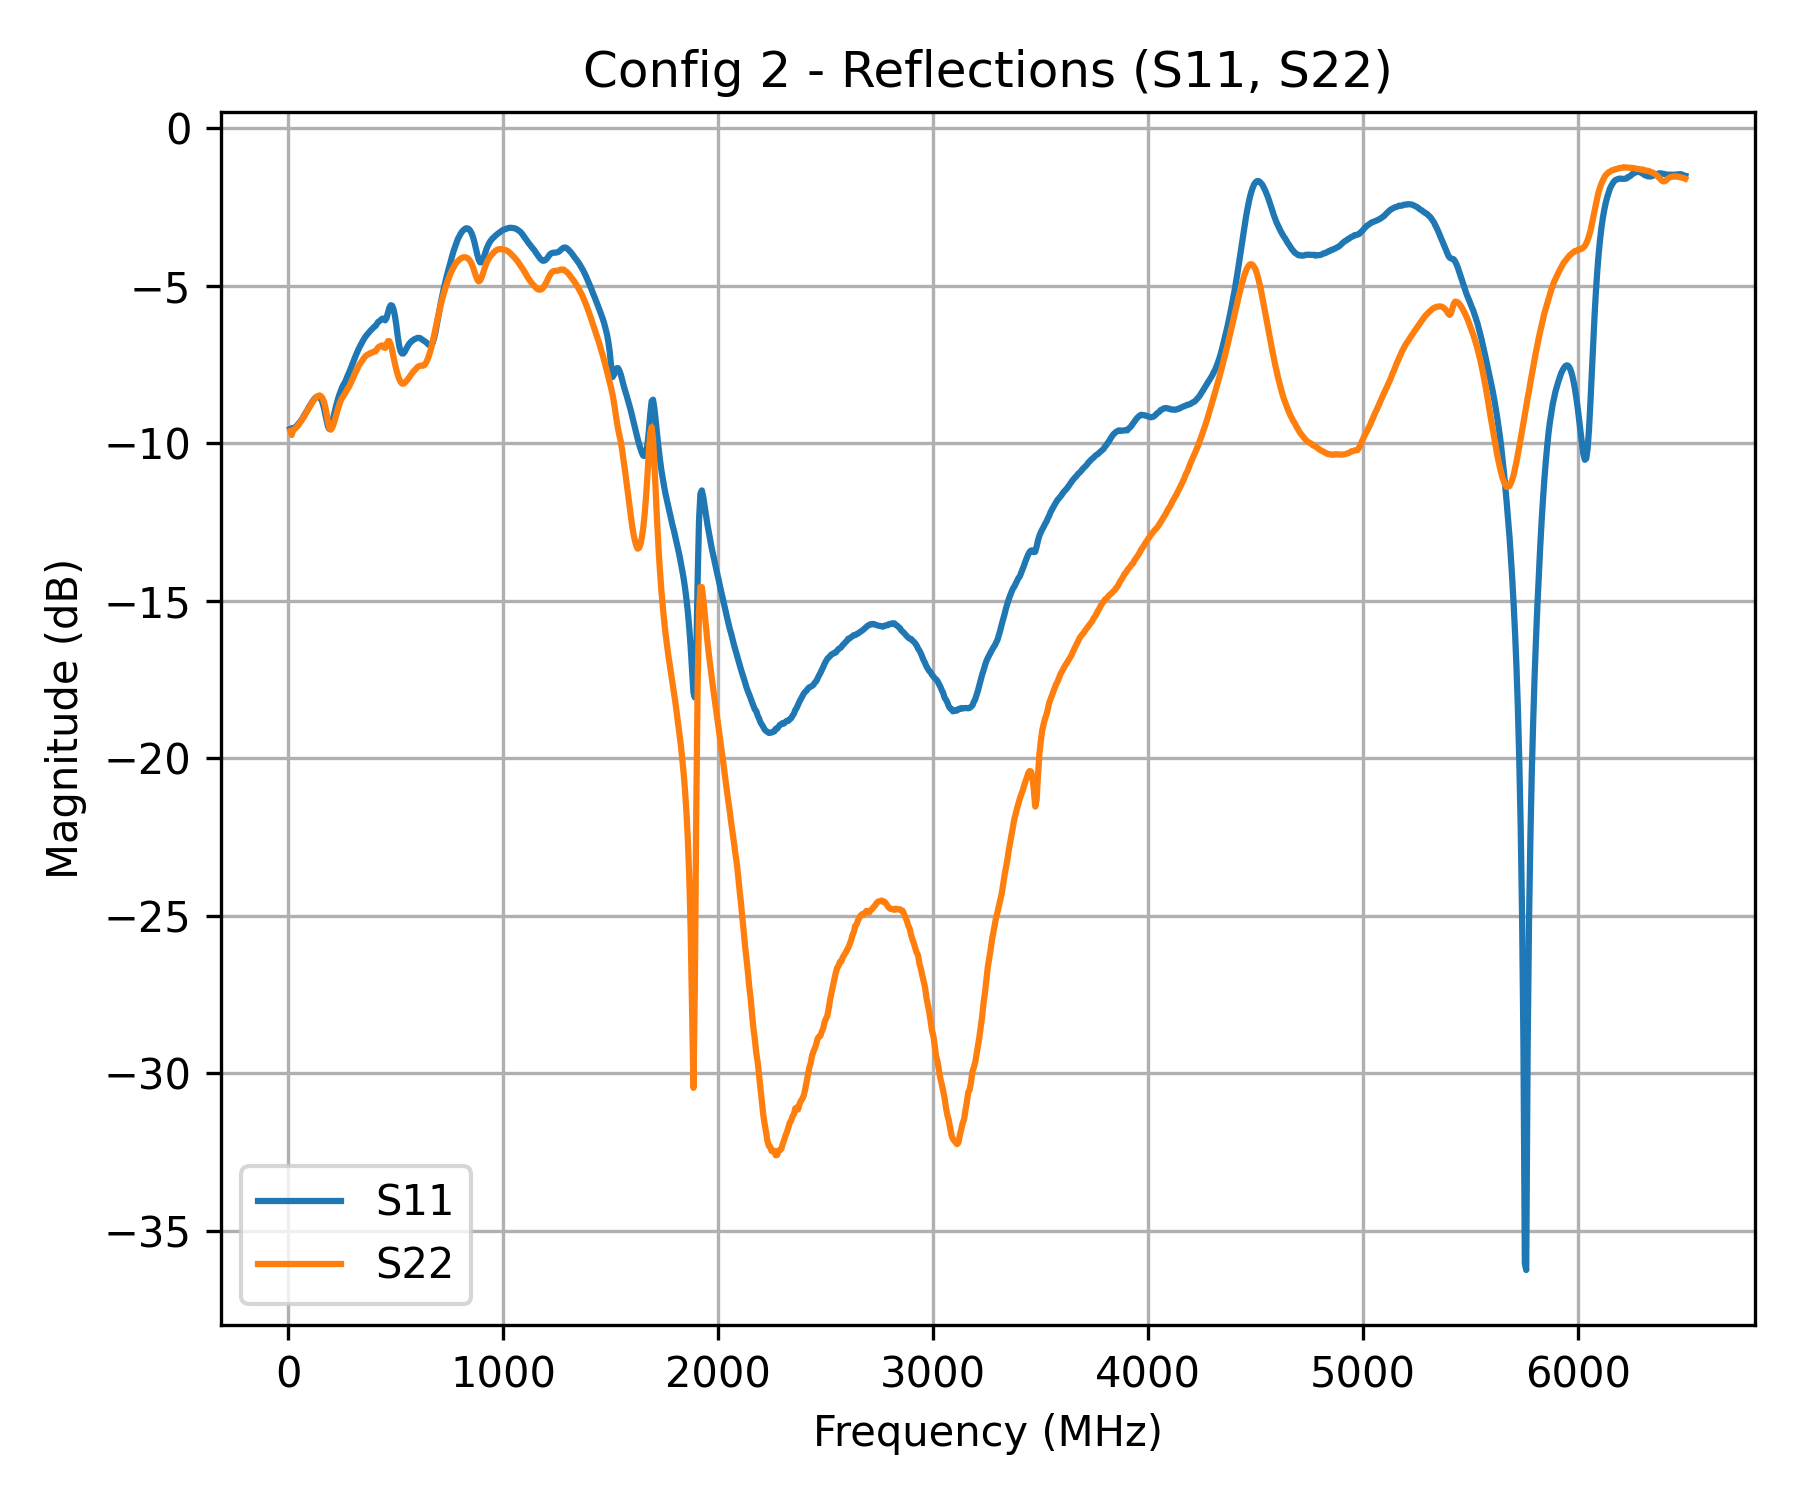
\includegraphics[width=0.6\linewidth]{Davides_Section/Circulator/plots/config2_reflection.png}
\caption{Reflection coefficients $S_{11}$ and $S_{22}$ for configuration 2.}
\label{fig:config2_reflection}
\end{figure}

Also in the second configuration the reflection coefficients indicate a generally acceptable matching, with some frequency regions showing deeper minima and therefore better impedance adaptation.

\begin{figure}[H]
\centering
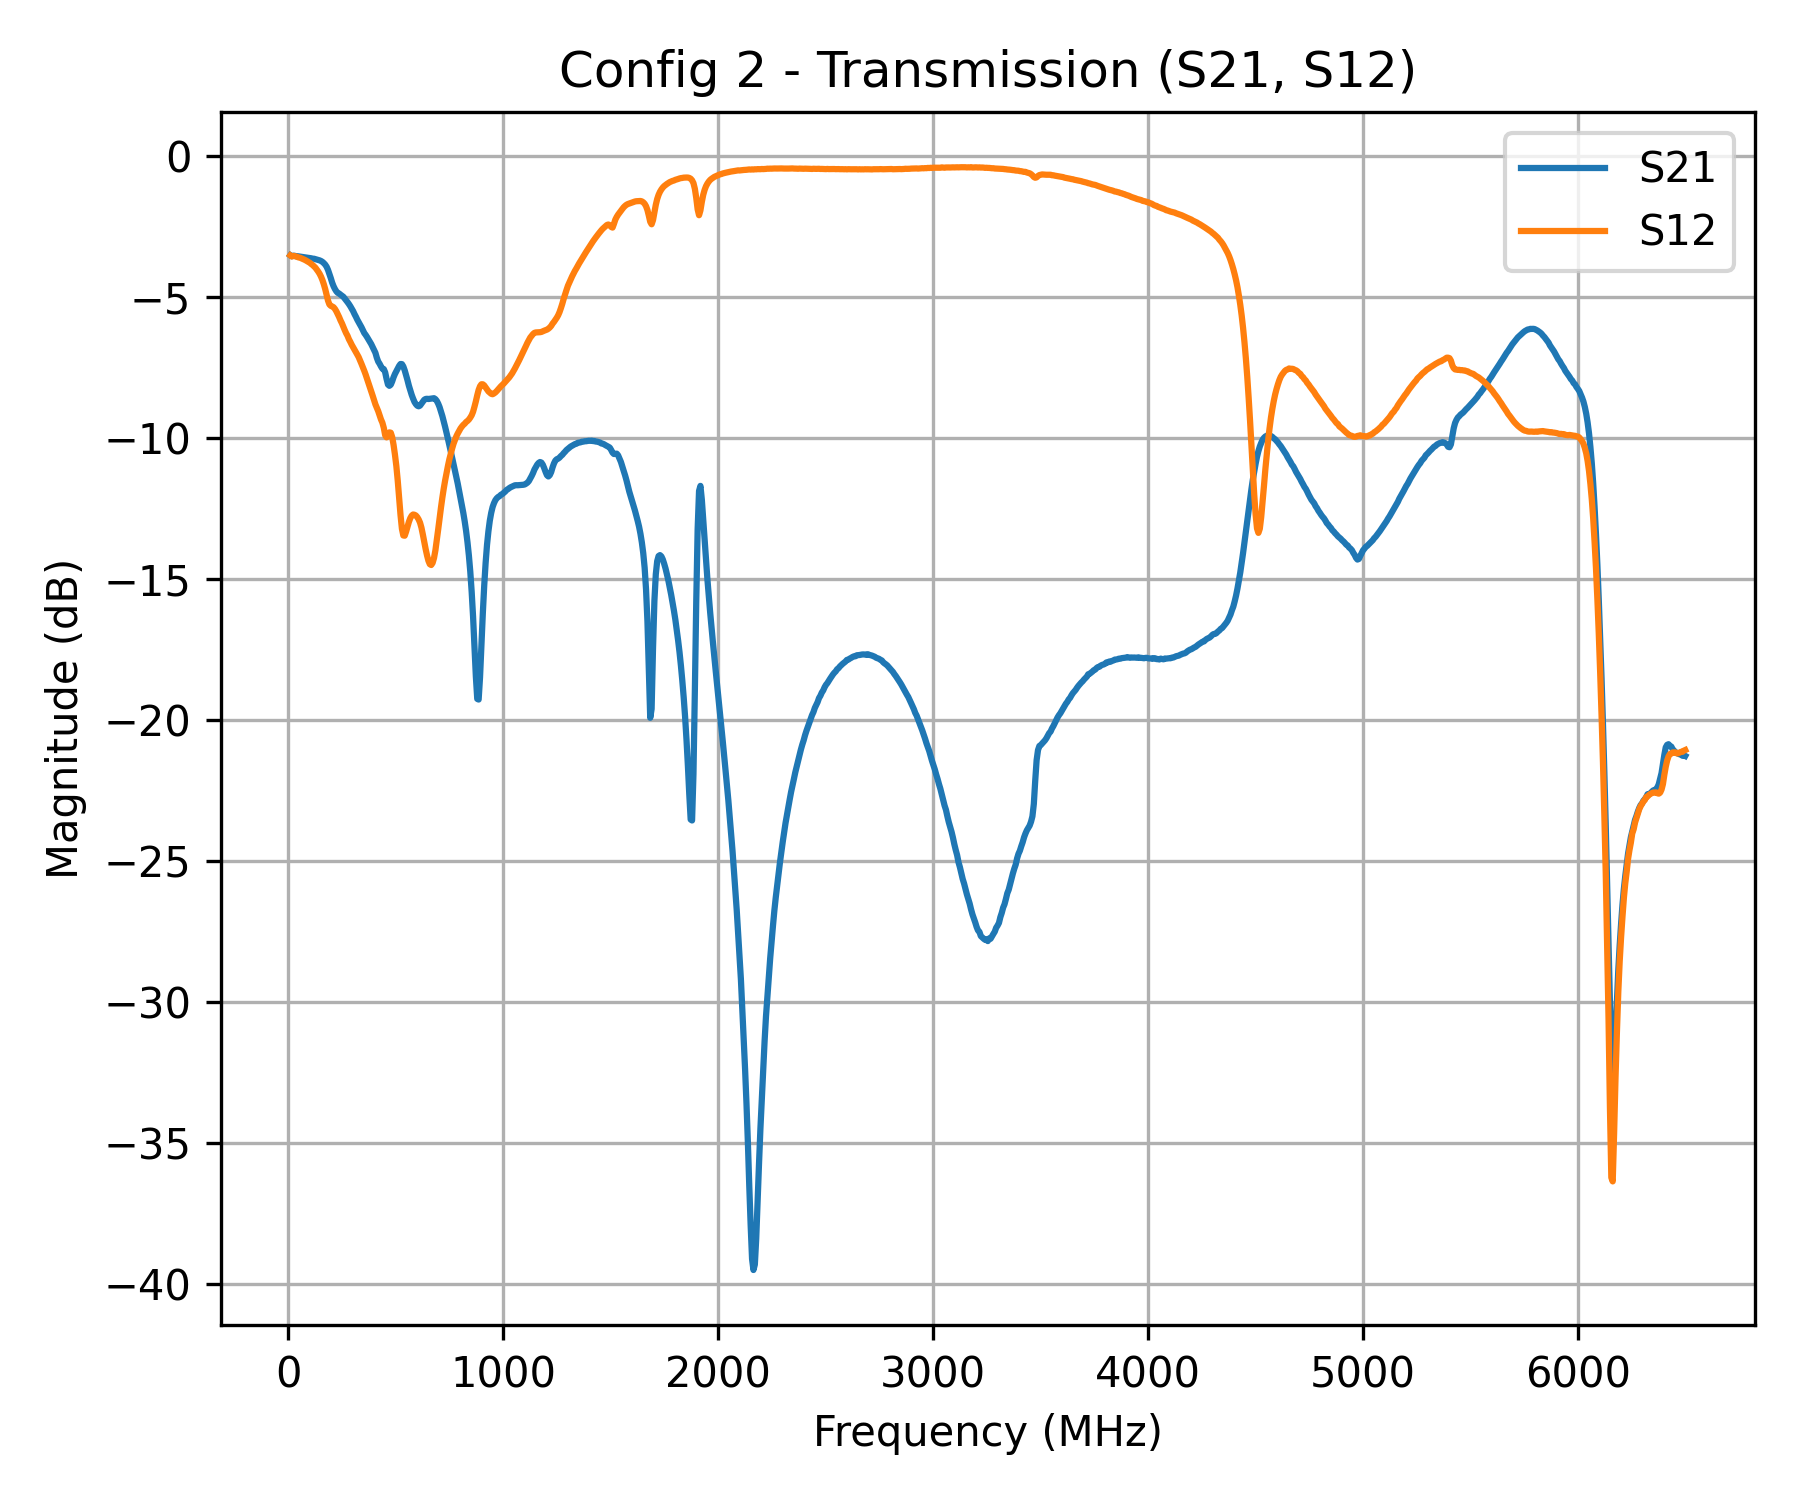
\includegraphics[width=0.6\linewidth]{Davides_Section/Circulator/plots/config2_transmission.png}
\caption{Transmission coefficients $S_{21}$ and $S_{12}$ for configuration 2.}
\label{fig:config2_transmission}
\end{figure}

In this case the connection of the ports is changed, and the measurements again highlight the directional nature of the circulator. One transmission coefficient is significantly larger than the opposite one over the useful frequency range, while the reverse direction remains attenuated. This confirms that the device does not behave reciprocally and that the transmitted power depends on the ordering of the ports.
terminating the third port with a matched $50\,\Omega$ load, it is possible to directly observe the cyclic routing of signals that characterizes the operation of a circulator.

\section{Physical Interpretation and Conclusion}

The circulator operates through a non-reciprocal propagation mechanism, meaning that the symmetry between forward and reverse signal transmission is intentionally broken. As a result, the signal is not allowed to propagate equally in both directions, but is instead routed along a preferred cyclic path among the three ports.

The purpose of the two measured configurations is precisely to make this behavior visible experimentally. By changing which pair of ports is connected to the VNA and terminating the remaining port with a matched load, it is possible to isolate the allowed transmission path and compare it with the forbidden one. In this way, the measurements directly show that the circulator routes power preferentially in one direction, while the opposite transmission is suppressed.

This is also the reason why the unused port must always be closed on a matched load: the load absorbs the power reaching that port and prevents it from being reflected back into the device, which would otherwise distort both reflection and transmission measurements.

The measurements confirm the non-reciprocal behavior of the circulator. In both configurations, the comparison between the transmission coefficients clearly shows that one direction is favored, while the opposite one is strongly attenuated. By measuring two different port configurations and properly terminating the third port with a matched $50\,\Omega$ load, it is therefore possible to directly observe the cyclic routing of signals that characterizes the operation of the device. The reflection data additionally indicate that the component remains reasonably well matched over a broad frequency range.
